\section{Datenformat}

\noindent In der Datei {\tt bays29.tsp} sind 29 bayrische Städte aufgeführt.
Der Kern der Datei ist die 29x29 Matrix, welche die Reisekosten zwischen
den den einzelnen Stäten beschreibt, dieser Städte-Graph ist zur Lösung
des Travelling-Salesman-Problems (TSP) gedacht.
Details des Aufbaus der Datei:

\begin{itemize}
  \item Header.\\
  Name, Problemtyp, Kommentar, Dimension des Problems bzw. der Matrix, Typ und Format der Kantengewichte
  \item Kantengewichte.\\
  29 x 29 Matrix mit den Reisekosten zwischen den einzelnen Städten als symmetrische Matrix, d.h. es handelt sich um einen ungerichteter Graphen.
  \item Positionen der Städte.\\
  Liste mit Stadtnummer und X-, Y-Koordinaten welche die Städtepositionen beschreiben.
\end{itemize}


\section{Testläufe mit tspVorlage.m}

Das {\tt tspVorlage.m} Skript wurde 15 mal ausgeführt und die Ergebnisse in
Tabelle \ref{testlaeufe} festgehalten und auf Abbildung \ref{fig.testlaeufe}
visualisiert.
Eine kleine Auswertung ergibt einen Mittelwert von 3077.93 km mit
einer Standardabweichung von 177.05 km.
Das Minimum beträgt 2764 km und das Maximum 3490 km.

Laut \cite{aufg} liegt die beste
Lösung\footnote{In der Software \emph{best objective value} genannt.},
also der kürzeste Weg für eine Rundreise, bei 2020 km.
Das bedeutet, hier gibt es noch Optimierungsbedarf.
In Kapitel \ref{testlaeufe} werden systematisch bessere Einstellungsparameter
gesucht, um einen möglichst kurzen Weg mit möglichst geringer Laufzeit zu finden.

\begin{table}[h]
\begin{tabular}{ | r | c | c | }
  \hline
  \# Iteration & kürzester Weg & in Generation \\
  \hline
  1  & 3324 & 288 \\
  2  & 3041 & 345 \\
  3  & 3180 & 388 \\
  4  & 3148 & 244 \\
  5  & 3102 & 372 \\
  6  & 2898 & 243 \\
  7  & 2980 & 287 \\
  8  & 2764 & 139 \\
  9  & 2982 & 307 \\
  10 & 3490 & 319 \\
  11 & 2974 & 293 \\
  12 & 3281 & 364 \\
  13 & 2991 & 313 \\
  14 & 2967 & 261 \\
  15 & 3047 & 353 \\
  \hline
\end{tabular}
\caption{Testläufe mit {\tt tspVorlage.m}}\label{testlaeufe}
\end{table}

\begin{figure}[h!]
  \centering
  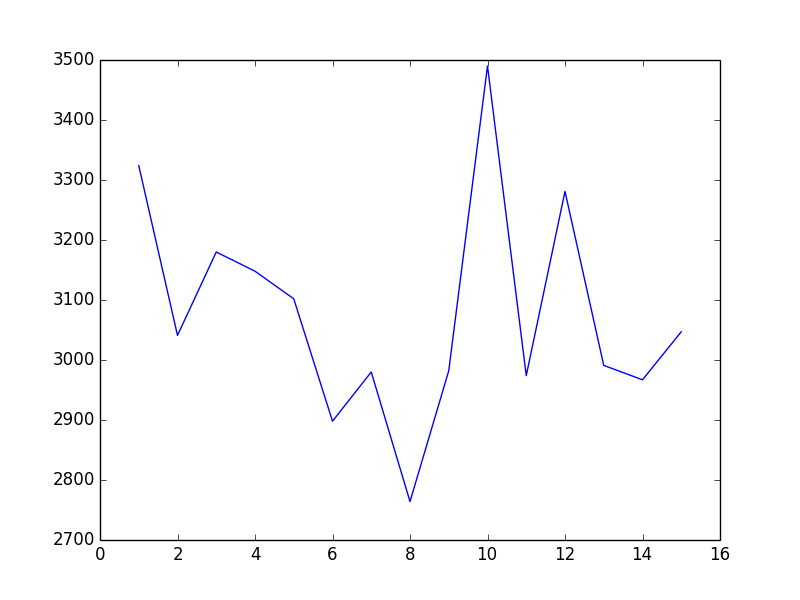
\includegraphics[width=1.0\textwidth]{Figures/tspVorlage.png}
  \caption{Testläufe mit {\tt tspVorlage.m}}\label{fig.testlaeufe}
\end{figure}


\section{Parameter und Optionen}

\begin{lstlisting}
geaoptset()
VariableFormat',            5 ...         % Use permutation variables  
NumberSubpopulation',   1 ...         % Number of subpopulation
NumberIndividuals',       50 ...        % Number of individuals per subpopulation
Selection.Name',          'selrws' ...  % Define the selection function
Selection.GenerationGap',   1 ...         % Set generation gap to 100%   
Recombination.Name',    'recpm' ...   % Define the recombination function
Mutation.Name',           'mutswap' ...   % Define the mutation functions
Mutation.Rate',           10 ...        % Define the mutation rate                   

Output.TextInterval',     100 ...       % Text output every 100 generations
Output.GrafikInterval',   100 ...       % Grafic results every 100 generations
Output.StatePlotInterval',  100       ...
Output.StatePlotFunction',  'plottsplib' ...
Termination.MaxGen',    400 ...       % Terminate after xx generations
Termination.Method',    1 ...         % Termination method to use

Output.SaveTextInterval',   0 ...                 % Text to File every xx generations
Output.SaveTextFilename', [FileNameBase '.txt'] ... % Filename of result file, absolut or relative path may be included
Output.SaveBinDataInterval',  0 ...                 % Binary Data to File every xx generations
Output.SaveBinDataFilename', [FileNameBase '.mat'] ... % Filename of binary file, absolut or relative path may be included


System.ObjFunFilename',   'objtsplib'
GeaOpt = geaoptset( GeaOpt , 'System.ObjFunAddPara', {TSPLIB_NAME});
% Get variable boundaries from objective function
   VLUB = geaobjpara(GeaOpt.System.ObjFunFilename, 1, GeaOpt.System.ObjFunAddPara)
   GeaOpt = geaoptset( GeaOpt , 'System.ObjFunVarBounds', VLUB); VLUB = [];

% Call main GEA function
   [xnew, GeaOpt] = geamain2(objfun, GeaOpt, VLUB, []);
\end{lstlisting}


\section{Automatisierte Testläufe}\label{testlaeufe}

In der Aufgabenstellung \cite{aufg} ist verlangt \emph{eine Konstellation zu finden,
unter der der Algorithmus möglichst gute Lösungen in möglichst kurzer Zeit} findet.
Um dies zu bewerkstelligen, müssen bessere Parametrisierungen für den Algorithmus
gefunden werden. Dazu wurde ein automatisiertes Testsystem aufgebaut, um
die Parameter systematisch abzusuchen sodass ideale Parametrisierungen
gefunden werden. Das Testsystem wird im Folgenden erklärt, die Ergebnisse
werden in Kapitel \ref{ergebnisse} präsentiert und analysiert.

Ergebnis von [xnew, GeaOpt] = geamain2()
xnew(1,:) liefert den besten Weg
GeaOpt.Run.BestObjectiveValue liefert die geringsten Kosten

\subsection{Ergebnisse}\label{ergebnisse}

\begin{table}[tbp]
\begin{tabular}{ | c || r | r | r | r | r | }
\hline
Parameter & \# Läufe & Mittelwert & Std.-Abw. & Laufzeit & Min, Max \\
\hline
   1.00 &  10 & 2515.70 &   83.09 &  127.44 & 2418, 2729 \\
   2.00 &  10 & 2650.80 &   55.88 &  128.35 & 2566, 2779 \\
   5.00 &  10 & 2814.90 &   40.74 &  129.43 & 2745, 2886 \\
  10.00 &  10 & 2956.10 &   66.79 &  129.32 & 2844, 3067 \\
  20.00 &  10 & 2942.30 &   59.01 &  130.21 & 2789, 3001 \\
  30.00 &  10 & 2918.00 &   88.64 &  129.95 & 2723, 3020 \\
\hline
\end{tabular}
\caption{Migration.Interval}
\end{table}


\begin{table}[tbp]
\begin{tabular}{ | c || r | r | r | r | r | }
\hline
Parameter & \# Läufe & Mittelwert & Std.-Abw. & Laufzeit & Min, Max \\
\hline
   0.01 &  10 & 2956.50 &   66.98 &  127.93 & 2858, 3030 \\
   0.02 &  10 & 2932.90 &   62.62 &  128.32 & 2823, 3054 \\
   0.05 &  10 & 2908.90 &   77.54 &  129.81 & 2789, 3015 \\
   0.10 &  10 & 2977.10 &   57.18 &  130.47 & 2912, 3079 \\
   0.15 &  10 & 2930.80 &   80.85 &  129.96 & 2759, 3043 \\
   0.25 &  10 & 2916.10 &   70.82 &  130.00 & 2761, 3021 \\
\hline
\end{tabular}
\caption{Migration.Rate}
\end{table}


\begin{table}[tbp]
\begin{tabular}{ | c || r | r | r | r | r | }
\hline
Parameter & \# Läufe & Mittelwert & Std.-Abw. & Laufzeit & Min, Max \\
\hline
   0.00 &  10 & 2938.20 &   63.43 &  131.35 & 2830, 3033 \\
   1.00 &  10 & 2914.40 &   65.73 &  129.25 & 2816, 3038 \\
\hline
\end{tabular}
\caption{Migration.Selection}
\end{table}


\begin{table}[tbp]
\begin{tabular}{ | c || r | r | r | r | r | }
\hline
Parameter & \# Läufe & Mittelwert & Std.-Abw. & Laufzeit & Min, Max \\
\hline
   0.00 &  10 & 2962.40 &   78.42 &  131.27 & 2813, 3078 \\
   1.00 &  10 & 2945.30 &   89.98 &  130.39 & 2776, 3044 \\
   2.00 &  10 & 2963.20 &   67.01 &  131.35 & 2835, 3044 \\
\hline
\end{tabular}
\caption{Migration.Topology}
\end{table}


\begin{table}[tbp]
\begin{tabular}{ | c || r | r | r | r | r | }
\hline
Parameter & \# Läufe & Mittelwert & Std.-Abw. & Laufzeit & Min, Max \\
\hline
  10.00 &  11 & 3604.36 &  156.64 &   -1.00 & 3271, 3838 \\
  20.00 &  11 & 3331.55 &  194.16 &   -1.00 & 3096, 3657 \\
  30.00 &  10 & 3235.10 &  174.55 &   -1.00 & 2960, 3569 \\
  50.00 &  10 & 3090.30 &  151.34 &   -1.00 & 2829, 3395 \\
  75.00 &  10 & 3005.70 &   88.17 &   -1.00 & 2851, 3181 \\
 100.00 &  10 & 2985.00 &   95.18 &   -1.00 & 2800, 3123 \\
 200.00 &  10 & 2990.50 &   90.44 &   -1.00 & 2862, 3181 \\
 300.00 &  10 & 2926.10 &   84.25 &   -1.00 & 2716, 3024 \\
 400.00 &  10 & 2925.10 &   59.14 &   -1.00 & 2838, 3020 \\
 500.00 &  10 & 2881.20 &   54.06 &   -1.00 & 2810, 2962 \\
 625.00 &  10 & 2872.10 &   81.27 &   -1.00 & 2772, 3028 \\
 750.00 &  10 & 2897.20 &   71.38 &   -1.00 & 2746, 2988 \\
1000.00 &  10 & 2858.20 &   85.99 &   -1.00 & 2694, 2987 \\
1250.00 &  10 & 2832.30 &   43.77 &   -1.00 & 2764, 2897 \\
1500.00 &  10 & 2847.10 &   78.61 &   -1.00 & 2648, 2963 \\
\hline
\end{tabular}
\caption{NumberIndividuals}
\end{table}


\begin{table}[tbp]
\begin{tabular}{ | c || r | r | r | r | r | }
\hline
Parameter & \# Läufe & Mittelwert & Std.-Abw. & Laufzeit & Min, Max \\
\hline
   1.00 &  10 & 3080.00 &  103.00 &   -1.00 & 2913, 3232 \\
   2.00 &  10 & 2993.90 &  173.72 &   -1.00 & 2695, 3297 \\
   3.00 &  10 & 2974.30 &   63.59 &   -1.00 & 2838, 3045 \\
   5.00 &  10 & 2916.70 &   99.34 &   -1.00 & 2779, 3068 \\
   7.00 &  10 & 2915.60 &   55.28 &   -1.00 & 2828, 2984 \\
  10.00 &  10 & 2878.90 &   72.28 &   -1.00 & 2719, 3004 \\
  15.00 &  10 & 2854.50 &   58.09 &   -1.00 & 2780, 2958 \\
  20.00 &  10 & 2867.50 &   93.64 &   -1.00 & 2689, 2974 \\
  30.00 &  10 & 2808.30 &   57.47 &   -1.00 & 2700, 2894 \\
  40.00 &  10 & 2836.00 &   71.85 &   -1.00 & 2711, 2924 \\
  50.00 &  10 & 2809.10 &   49.99 &   -1.00 & 2742, 2876 \\
\hline
\end{tabular}
\caption{NumberSubpopulation}
\end{table}



